% ######################################################################### %
% ------------------------------------------------------------------------- %
%                    Distance dependent connectivity
% ------------------------------------------------------------------------- %
% ######################################################################### %


\section{Distanc-dependent Connectivity}
\label{sec:distance_connectivity}



In Gilbert's random graph model $G(n,p)$,
%------------------------------------------------ 
\marginpar{random graph
  models in Section~\ref{sec:random_graph_theory}}
%------------------------------------------------
probability of connection $p$ is independently chosen and a fixed
value for all vertex pairs. The anisotropic geometric graph model
introduced in Section~\ref{sec:anisotropic_network_model} is itself a
random graph model - node positions as well as preferred directions of
connection are uniformly at random distributed. In contrast to
Gilbert's model however, neither is the probability of connection
between a given vertex pair independent of the realization of other
edges in the graph, nor is it a fixed value - probabilities strongly
depend on internode distance in the anisotropic geometric graph model
introduced.

Analyzing dependencies in the anisotropic model, specifically by
identifying prevalent patterns of connectivity and relating these
modes of non-randomness to biological findings, is the main focus of
Chapter~\ref{ch:structural_aspects}. However, such structural
correlations may not necessarily be an inherent feature of the
network's anisotropy - distance dependent connectivity alone, as
imposed by the model's specific geometry, may be the cause for
emerging dependencies. It is therefore a crucial initial task to map
the anisotropic model's distance dependent connection
probability. Inferring connection probability as a function of
internode distance and comparing it with computational results, in
this section we explore distance connectivity of the anisotropic
network model, securing a vital component in the analysis of
structural features.

\begin{theorem} \label{theorem:distance_prof} Let $(G,\Phi, a)$
  represent an arbitrary realization of the anisotropic random graph
  model $G(n,w)$. Define $C:[0,\sqrt{2}] \to [0,1]$ as the
  distance-dependent connection probability profile of $(G,\Phi)$,
  that is such that $C(x)$ is the probability that for a vertex pair
  $(v,v') \in V(G)^2\setminus\Delta_{V(G)}$ in distance $x =
  \norm{\Phi(v)-\Phi(v')}$ the vertex $v$ projects to vertex
  $v'$. Then
  \[
    C(x) = \begin{cases}%
             \frac{1}{2} & \mathrm{for} \,\, x\le w/2 \\
             \frac{1}{\pi}
             \operatorname{arcsin}\left(\frac{w}{2x}\right) &
             \mathrm{for} \,\, x >  w/2. %
           \end{cases}
  \]
\end{theorem} 

\begin{proof}
  Let $v,v'$ be a pair of vertices in $V(G)^2 \setminus \Delta_{V(G)}$
  in Euclidean distance $x$ of each other. The vector difference
  $\Phi(v')-\Phi(v)$ may then be written as $x e^{i\theta}$, with $0
  \leq \theta < 2\pi$. We have 
  \[
    R_{-\alpha(v)} xe^{i\theta} = xe^{i(\theta - \alpha(v))}.
  \]
  Only for suitable combination of $\theta$ and $\alpha(v)$ an edge
  from $v$ to $v'$ exists. Assuming $\alpha(v)$ fixed, we calculate
  the probability of connection depending on the random choice of
  $\theta$. We can assume $\alpha(v) = 0$, otherwise the same argument
  holds for $\theta' = \theta - \alpha(v)$.

  From \ref{def:anisotropic_geometric_graph} we obtain the necessary and
  sufficient conditions
  \[
   x \cos \theta \geq 0 \quad \mathrm{and} \quad \abs{x\sin \theta}
  \leq \frac{w}{2}.
  \]
  Choosing uniformly at random $\theta$ in the range of $[0,2\pi)$,
  the first condition is satisfied with a probability of
  $\frac{1}{2}$. Consider for the second condition $\theta \in
  [0,\pi)$. We have 
  \[ 
  \sin \theta \leq \frac{w}{2x},
  \]
  and for $x \leq \frac{w}{2}$ the inequality holds for all $\theta$
  by definition of $\sin \theta$. In the case of $x > \frac{w}{2}$, we
  note that for the first condition to hold $\theta$ must already be in
  $[0,\frac{\pi}{2})$ and can thus write the second condition $\theta$ as
  \[
    \theta \leq \operatorname{arcsin}\frac{w}{2x},
  \]
  yielding $C(x)$ by combining the considerations above and using the
  symmetry of sine for $\theta$ in the third and fourth quadrant.
  % 
\end{proof}

\vspace{0.2cm}%??
\begin{figure}[H] 
  \centering 
  \makebox[0.8\textwidth]{%
    \begin{overpic}[width=0.35\textwidth]{%
        tikz/geomtr_prb_05.pdf}%
      \put(3,92){\small\textbf{A}}
    \end{overpic}
    \hfill
    \begin{overpic}[width=0.35\textwidth]{%
        tikz/geomtr_prb.pdf}% 
      \put(3,92){\small\textbf{B}}
    \end{overpic}  
  }%
  \caption{\textbf{Illustrating the proof of
      Theorem~\ref{theorem:distance_prof}} Distance-dependent
    connectivity profile $C(x)$ in an anisotropic geometric graph
    calculated from geometric dependencies. \textbf{A)} In the case of
    $x\leq \nicefrac{w}{2}$, target $v'$ may be located anywhere on the
    shown semicircle and therefore receives input from $v$ with
    probability $\nicefrac{1}{2}$. \textbf{B)} For $x > \nicefrac{w}{2}$,
    suitable positions for target $v'$ are dependent on $x$. The
    geometric relation $\sin \theta = \nicefrac{w}{2x}$ leads to the
    distance-dependent connectivity profile as described in
    Theorem~\ref{theorem:distance_prof}.}
  \label{fig:geomtr_prb}
\end{figure}


We can verify this result by extracting the distance-dependent
connection probabilities in the sample graphs created in
Section~\ref{sample_graphs}. Combining data of all 25 graphs, we find
that connection probabilities perfectly match the theoretical
prediction (\autoref{fig:distance_theory_compare}). Additionally we're
%------------------------------------------------ 
\marginpar{distance-dependent sample graphs as reference}%
\label{distance_dependent_sample}%
%------------------------------------------------
able to extend the reference sample graphs by distance-dependent
networks (Definition~\ref{def:distance_dependent_graph}). Using
Theorem~\ref{theorem:distance_prof} in conjunction with the sample
graph parameter set ($N=1000$, $s=100$\footnote{The generalization of
  Theorem~\ref{theorem:distance_prof} to allow for arbitrary
  side-length $s$ is trivial and omitted here}, $w=25.2$) we easily
obtain the expected distance-dependent connectivity profile for the
created sample graphs and, using this profile, generate purely
distance-dependent networks\footnote{label:
  \smtcite{N1000-dist\char`_depend-flat\char`_graph-00-24.xml.gz}}. Being
highly interested in structural features not explained by
distance-dependent connectivity, the numerical analysis in this work
will heavily rely on these networks to identify aspects that are
inherent to the anisotropy in connectivity.


\begin{figure}[H]
  \centering
  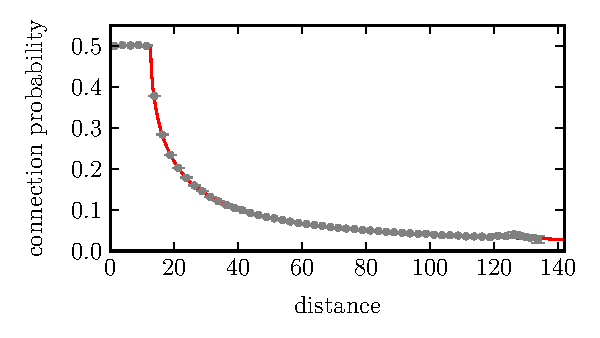
\includegraphics[width=0.8\linewidth]{%
    plots/dbffa88e.pdf} 
  \captionsetup{skip=0pt}
  \caption{\textbf{Predicted distance-dependent connection probability
      profile is matched by numerical results} Averaging
    distance-dependent connection probabilities over the 25 sample
    graphs, we find the expected profile calculated in
    Theorem~\ref{theorem:distance_prof} is matched perfectly by the
    numerical results. (\smtcite{dbffa88e}) }
  \label{fig:distance_theory_compare}
\end{figure}






%%% Local Variables: 
%%% mode: latex
%%% TeX-master: "../dplths_document"
%%% End: 
